\documentclass{paper}

\usepackage{amsmath,amssymb,amsfonts, listings, fancyhdr, stmaryrd, array, tikz}
\usepackage[many]{tcolorbox}
\usepackage[a4paper, total={170mm,257mm}, left=20mm, top=20mm]{geometry}
\newtheorem{prop}{Proposition}
\newtheorem{defi}{Definition}
\newtheorem{preuve}{Preuve}

\newcolumntype{C}{>$c<$}
\tcolorboxenvironment{prop}{enhanced, borderline={0.8pt}{0pt}{blue}, borderline={0.4pt}{2pt}{cyan}, boxrule=0.4pt, colback=white, coltitle=black, sharp corners}
\tcolorboxenvironment{defi}{ enhanced, borderline={0.8pt}{0pt}{red}, borderline={0.4pt}{2pt}{orange}, boxrule=0.4pt, colback=white, coltitle=black, sharp corners}
\tcolorboxenvironment{preuve}{ enhanced, borderline={0.8pt}{0pt}{green}, borderline={0.4pt}{2pt}{lime}, boxrule=0.4pt, colback=white, coltitle=black, sharp corners}

\pagestyle{fancy}
\fancyhead[C]{TIPE 25/26 - Dorian GIL}

\begin{document}
\setlength{\headheight}{13.07225pt}
\addtolength{\topmargin}{-1.07225pt}

\section*{Méthode des tableaux : Optimisation pour des formules de la forme alternée}


Forme proposition pour accelerer methode tableau
memoisation des propositions (SQL, dictionnaire, serialisation ?)

\tableofcontents

\section{Logique Propositionelle}
\subsection{Definition}
\begin{defi}
La \textit{logique propositionelle} est un type de logique où les formules sont obtenus par des variables propositionelles reliées par des connecteurs.
\end{defi}
\begin{defi}[Modèle]
    Un \textit{modèle} d'une formule $\phi$ est une valuation qui rend vraie cette formule. On note l'ensemble des modèles de $\phi$ par:
    $$Mod(\phi) := \{v\in Val | v \vDash \phi\}$$
    $Val$ étant l'ensemble des valuations de $\phi$ et $v \vDash \phi$ signfiant que la valuation $v$ satisfait $\phi$
\end{defi}
\begin{defi}[Conséquence Logique]
    Une formule $\phi$ est \textit{conséquence logique} d'une formule, notée $\psi$ si $Mod(\psi) \subseteq Mod(\phi)$. On note cela $\psi \vDash \phi$
\end{defi}

On note $\mathcal{V}$ un vocabulaire qu'on définie par $\mathcal{V} := \{p, q,\dots, \lnot, \land, \lor, \implies, \Leftrightarrow, (,) \}$ et $\mathcal{V}$* l'ensemble de toutes les expressions que l'on peut former avec le vocabulaire $\mathcal{V}$
\begin{defi}[Système formel]
    Un système formel est défini par un tuple $(\mathcal{V}, \mathcal{E}, \mathcal{A}, \mathcal{R})$, tel que:
    \begin{itemize}
        \item $\mathcal{V}$ est un ensemble de symboles
        \item $\mathcal{E}$ est un ensemble d'expressions bien formées dans $\mathcal{V}$*
        \item $\mathcal{A}$ est un ensemble d'axiomes ($\mathcal{A} \subset \mathcal{E}$)
        \item $\mathcal{R}$ est un ensemble de règles de déduction de la forme: $r_i : f_1, f_2,\dots, f_n \vdash g$ avec $f_i, g \in \mathcal{E}$
    \end{itemize}
\end{defi}

\begin{defi}[Déduction ou preuve]
    Soit un système SF, une preuve de $c_p$ à partir de $h_1,\dots,h_n$ dans SF qu'on note $h_1,\dots, h_n \vdash c_p$
    toute suite $c_1,\dots,c_p$ telle que $\forall i\in\mathcal{N} | 1 \leq i \leq p$, $c_i$ est un des suivants:
    \begin{itemize}
        \item Un axiome
        \item Une hypothèse
        \item Obtenu par application d'une règle $r_i$ telle que $c_{i_1},\dots c_{i_k} \vdash c_i$ où $ i_1,\dots,i_k < i$
    \end{itemize}
\end{defi}

On note $n\in\mathbb{N}^*$
\begin{defi}
    \textit{La méthode des tableaux} consistent à prouver une assertion $B$ ayant pour hypothèse $(A_n)$ en montrant
    que $\{A_1,\dots,A_n, \lnot B\}$ est insatisfaisable (Cela revient à montrer qu'une implication est vraie car sa négation ne peut être vraie)
    i.e $((A_1,\dots,A_n)\implies B) \Leftrightarrow Mod(\lnot((A_1,\dots,A_n)\implies B)) = \emptyset \Leftrightarrow Mod((A_1,\dots,A_n)\land \lnot B) = \emptyset$.
\end{defi}

Le procédé consiste donc à séparer les formules logiques complexes en plus petite formule jusqu'à que des pairs complementaires de litteraux ($a$ et $\lnot a$) soit extrait ou qu'on ne peut plus simplifier la formule.
Pour cela, on doit définir quelques concepts sur les arbres.

\begin{defi}[Arbre de déduction]
    Arbre dont les sommets sont composés de formule, qui sont soit une hypothèse à la racine de l'arbre, soit une formule obtenue par l'application d'une règle sur une formule présente dans la même branche plus proche de la racine.
\end{defi}

\begin{defi}[Branche fermée]
    Une branche est fermée si elle contient $\phi$ et $\lnot\phi$
\end{defi}

\begin{defi}[Arbre fermé]
    Un arbre de déduction est fermé si toutes les branches le sont.
\end{defi}

\subsection{Principe}
Pour ainsi en déduire si une formule $\phi$ est vrai ou non, on adopte des règles qu'on applique sur un arbre de déduction.
\begin{itemize}
    \item On place $\lnot\phi$ dans la racine de l'arbre.
    \item On applique les règles $(R_x)$ suivantes à chaque branche non fermé de l'arbre
    \item Si l'arbre est in fine fermé, alors $\phi$ est vrai
\end{itemize}

Les règles $(R_x)$ dites Smullyan-style sont:

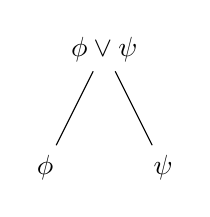
\begin{tikzpicture}
\node {$\phi\lor\psi$}
    child {node {$\phi$}}
    child {node {$\psi$}};
\end{tikzpicture}
$(R_\lor)$
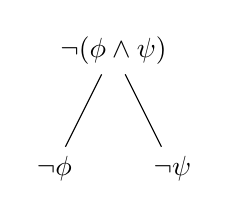
\begin{tikzpicture}
\node {$\lnot(\phi\land\psi)$}
    child {node {$\lnot\phi$}}
    child {node {$\lnot\psi$}};
\end{tikzpicture}
$(R_{\lnot\land})$
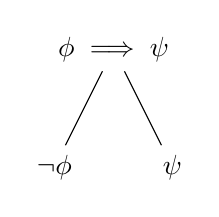
\begin{tikzpicture}
\node {$\phi\implies\psi$}
    child {node {$\lnot\phi$}}
    child {node {$\psi$}};
\end{tikzpicture}
$(R_{\implies})$
\begin{tikzpicture}
\node {$\lnot\lnot\phi$}
    child {node {$\phi$}};
\end{tikzpicture}
$(R_{\lnot\lnot})$
\begin{tikzpicture}[level distance=8mm]
\node {$\phi\land\psi$}
    child {node {$\phi$} edge from parent }{
    child {node {$\psi$} edge from parent[draw=none]}};
\end{tikzpicture}
$(R_{\land})$

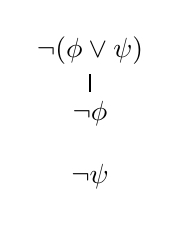
\begin{tikzpicture}[level distance=8mm]
\node {$\lnot(\phi\lor\psi)$}
    child {node {$\lnot\phi$} edge from parent }{
    child {node {$\lnot\psi$} edge from parent[draw=none]}};
\end{tikzpicture}
$(R_{\lnot\lor})$
\begin{tikzpicture}[level distance=8mm]
\node {$\lnot(\phi\implies\psi)$}
    child {node {$\phi$} edge from parent }{
    child {node {$\lnot\psi$} edge from parent[draw=none]}};
\end{tikzpicture}
$(R_{\lnot\implies})$
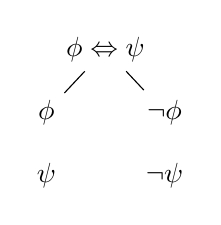
\begin{tikzpicture}[level distance=8mm]
\node {$\phi\Leftrightarrow\psi$}
    child {node {$\phi$} 
        child {node {$\psi$} edge from parent[draw=none]}}
    child {node {$\lnot\phi$}
        child {node {$\lnot\psi$} edge from parent[draw=none]}};
\end{tikzpicture}
$(R_{\Leftrightarrow})$
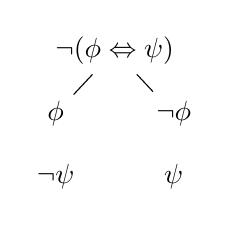
\begin{tikzpicture}[level distance=8mm]
\node {$\lnot(\phi\Leftrightarrow\psi)$}
    child {node {$\phi$} 
        child {node {$\lnot\psi$} edge from parent[draw=none]}}
    child {node {$\lnot\phi$}
        child {node {$\psi$} edge from parent[draw=none]}};
\end{tikzpicture}
$(R_{\lnot\Leftrightarrow})$

Dans les cas où on trouve dans une même branche $a$ et $\lnot a$, on ferme la branche, si l'arbre devient fermé, alors $\lnot\phi$ est forcement faux, donc $\phi$ est vrai.
a1 et (a2 ou a3)
\begin{prop}
    Soit $\Psi$ un ensemble d'hypothèse et $\phi$ une formule, on note $\Psi\vdash\phi$ l'existence d'un arbre fermé pour $\Psi\cup\{\lnot\phi\}$.
    $$\Psi\vdash\phi \Leftrightarrow \Psi\vDash\phi$$
    Autrement dit, appliqué la méthode des tableaux est équivalent à prouver cette formule
\end{prop}
La preuve de cette proposition permet de prouver la correction de l'implémentation de base.

\subsection{Optimisation pour les formules de forme alternée}

\begin{defi}
Soit $n\in\mathbb{N}^*$ $(\alpha_k)_{k\in[|1, n|]}$, une formule $\phi$ est de forme alternée ssi
$$\phi := \alpha_1 \land (\alpha_2 \lor (\alpha_3 \land (\dots (\alpha_n))))$$
\end{defi}
On gardera les parenthèses dans la suite pour garder le coté intuitiff de cet ecriture

On remarque une CNS pour que ce genre de formule soit vrai:
\begin{prop}
    $\phi$ de forme alternée est vrai ssi:
    $$(\exists k\in\mathbb{N}^*, \alpha_{2k-2} \text{ OU n impair}\implies\alpha_n \text{ avec } k=\frac{n-1}{2})\text{ ET } \forall i\in[|1, k|], \alpha_{2i-1}$$
\end{prop}

\begin{preuve}
    $(\impliedby)$ Immédiat
    
    $(\implies)$ Supposons $\phi$ de forme alternée vrai:
    $\alpha_1$ est forcement vrai, deux possibilités :
    soit $\alpha_2$ est vrai, soit $\alpha_3\land(\dots)$ est vrai. Dans le deuxième cas, on repète le raisonnement sur $\alpha_3\land(\dots)$ qui est bien de forme alternée.
    
    Deux cas de figure:
    \begin{itemize}
        \item On arrête donc le processus dès que un litteral indéxée par un nombre pair est vrai.
        Dans ce cas là, tout les indéxées impair précedents sont aussi vrai.
        \item Si aucun litteral pair est vrai, alors $n$ est impair sans quoi $\phi$ n'est pas vrai car $\alpha_n$ doit être vrai. 
        On en déduit que tout les litteraux impairs sont vraies, donc la formule est vrai.
    \end{itemize}    
\end{preuve}
Mais on cherche une CNS de satisfaisabilité.







\section{Logique du 1er ordre (FAIT PLUS TARD)}
La logique propositionelle étant mathématiquement limité, on se propose l'utilisation de la logique du 1er ordre.
Cela nous permettra ainsi d'étudier Zenon, un prouveur d'automatique de theorème.
\begin{defi}
    La \textit{logique du 1er ordre} est un type de logique qui en plus des élements de la logique propositionelle permet l'utilisation de
    quantificateurs et de \textit{termes}.
\end{defi}

\begin{defi}
    Soit un ensemble infini de variables $X = \{x,y,x_1,x_2,\dots \}$ et un ensemble $\mathcal{F}=\{c,f,g,\dots \}$ de symboles de fonction (autrement appelé signature).
    On rappelle que l'arité d'un symbole est son nombre d'argument.
    Les termes sont définis par induction:
    \begin{itemize}
        \item $\forall x\in X, x$ est un terme
        \item Tout symbole d'arité $0$ (les constantes) est un terme
        \item $f(t_1,\dots,t_n)$ est un terme ssi $f$ est un symbole d'arité $n$ et $t_1,\dots,t_n$ sont des termes
    \end{itemize} 
    On note $\mathcal{T}(\mathcal{F}, X)$ l'ensemble des termes sur $\mathcal{F}$ et $X$.
\end{defi}

\end{document}